\documentclass[12pt]{article}

\usepackage[T1]{fontenc} %US-ASCII-Codierung für westeuropäische Sprachen
\usepackage[a4paper,width=150mm,top=35mm,bottom=25mm,bindingoffset=6mm]{geometry} %here you define the geometry of the page 
\usepackage[utf8]{inputenc} %choose utf8 encoding
%\usepackage{lmodern}
%\usepackage{times} %here we use times new roman
\usepackage[english]{babel}

%Algorithms
\usepackage{algorithm}
\usepackage[noend]{algpseudocode}
\algnewcommand\algorithmicinput{\textbf{Input:}}
\algnewcommand\algorithmicoutput{\textbf{Output:}}
\algnewcommand\Input{\item[\algorithmicinput]}%
\algnewcommand\Output{\item[\algorithmicoutput]}%
\usepackage{transparent} %transparence in color
%indent within algorithmic
\usepackage[table, dvipsnames]{xcolor}
\usepackage[autostyle]{csquotes} %for quotation marks
\usepackage{enumitem} %for lists
\usepackage{graphicx} %for graphics
\usepackage{float}
\usepackage{mathrsfs}
\usepackage{amsmath} %math formula
\usepackage{amssymb}
\usepackage{booktabs}
\usepackage{url} %für URLs
\usepackage{breakurl} %brake URLs into separate lines if tehy are too long
\usepackage[breaklinks, hidelinks]{hyperref}
%make hidelinks applicabale

\usepackage{array}
\newcolumntype{P}[1]{>{\centering\arraybackslash}p{#1}}
\newcolumntype{M}[1]{>{\centering\arraybackslash}m{#1}}
\usepackage{listings} % to insert code
\usepackage{multirow} % merge cells
\usepackage{siunitx} % for \num{1e-10}
\usepackage{subcaption} % for side by side pictures
\usepackage{setspace}
%\usepackage[paper=a4paper,left=40mm,right=20mm,top=35mm,bottom=25mm]{geometry}
\onehalfspacing %hier setze ich 1.5 Zeilenabstand fest 
\usepackage{lscape} %Tabelle drehen
\usepackage{longtable} %for vertical table
\linespread{1.2}
\usepackage{etoolbox}
\usepackage[font={small}]{caption}
\usepackage{courier} %computer language font 
\setcounter{tocdepth}{2}
\graphicspath{{figures/}}

%\usepackage[acronym, toc]{glossaries} 
\usepackage[nonumberlist,acronym, toc, nogroupskip]{glossaries-extra}

\newglossaryentry{pi}{name = PI, description = {Artificial Intelligence}}

\makeglossaries
\newacronym{ai}{AI}{Artificial Intelligence}

\makeglossaries
\newacronym{rl}{RL}{Reinforcement Learning}

\makeglossaries
\newacronym{irl}{IRL}{Inverse Reinforcement Learning}

\makeglossaries
\newacronym{mdp}{MDP}{Markov Decision Process}

\makeglossaries
\newacronym{pomdp}{POMDP}{Partially Observable Markov Decision Process}

\makeglossaries
\newacronym{psr}{PSR}{Predictive State Representation}
\makeglossaries
\newacronym{rnn}{RNN}{Recurrent Neural Network}

\makeglossaries
\newacronym{lstm}{LSTM}{Long-Short Term Memory}

\makeglossaries
\newacronym{gru}{GRU}{Gated Recurrent Unit}

\makeglossaries
\newacronym{mle}{MLE}{Maximum Likelihood Estimation}

\makeglossaries
\newacronym{dqn}{DQN}{Deep Q-Learning Network}

\makeglossaries
\newacronym{ilp}{ILP}{Inductive Logic Programming}

\makeglossaries
\newacronym{bdi}{BDI}{Belief-Desire-Intention Model}

\makeglossaries
\newacronym{cpb}{CPB}{Case-Supported Principle-Based Paradigm}

\makeglossaries
\newacronym{id3}{ID3}{Iterative Dichotomiser 3}

\makeglossaries
\newacronym{ebb}{EBB}{Ethical Black Box}

\makeglossaries
\newacronym{mtt}{MTT}{Moral Turing Test}

\makeglossaries
\newacronym{cmtt}{cMTT}{Comparative Moral Turing Test}
 
\makeglossaries
\newacronym{tt}{TT}{Turing Test}

\makeglossaries
\newacronym{nn}{NN}{Neural Network}

\makeglossaries
\newacronym{agi}{AGI}{Artificial General Intelligence}

\makeglossaries
\newacronym{me}{ME}{Machine Ethics}

%singular \gls
%plural \glspl

%%%%%%%%%%%%%%%%%%%%%%%%%%%%%%%%%%%%%%%%%%%%%%%%%%%%%%%%%%%%%%%%%%%%

\setlength\parindent{0pt}


% Bibliography_preamble
%\usepackage[backend=biber,style=authoryear, autocite=inline]{biblatex}
%\addbibresource{ref.bib}
\usepackage[round]{natbib} %bibliography


\begin{document}

% Title
\begin{titlepage}
\newgeometry{left=2cm,right=2cm,top=2cm,bottom=2cm,bindingoffset=5mm}
\newcommand{\HRule}{\rule{\linewidth}{0.5mm}} % Defines a new command for the horizontal lines, change thickness here

\center % Center everything on the page
 
%----------------------------------------------------------------------------------------
%	HEADING SECTIONS
%----------------------------------------------------------------------------------------

\textsc{\LARGE Technische Universität Berlin}\\[0.5cm] 
\textsc{\large Quality \& Usability Lab, Faculty IV}\\[0.5cm] % Name of your university/college

%Include the logo

\includegraphics[scale=0.5]{figures/tub_logo.png}\\

\vspace{1cm}
%----------------------------------------------------------------------------------------
%	TITLE SECTION
%----------------------------------------------------------------------------------------

\HRule \\[0.4cm]
{ \Large \bfseries Here comes your main title \vspace{0.5cm} \\
\normalsize Here comes your subtitle}\\[0.3cm] % Title of your document
%{ \large \bfseries Opportunities and Tensions}\\[0.4cm] % Title of your document

\HRule \\[1.5cm]
 
%----------------------------------------------------------------------------------------
%	AUTHOR SECTION
%----------------------------------------------------------------------------------------
\textsc{\large Master/Bachelor thesis}\\[0.5cm] % Minor heading such as course title
%\begin{minipage}{0.3\textwidth}
\vspace{2cm}

\begin{minipage}{0.5\textwidth}
\begin{flushleft} \large
\emph{Author:} Your Name\\
\emph{Matrnr}.: fill in your matriculation number\\
\emph{Address}: your address \\
\emph{E-Mail}: your email\\
\end{flushleft}
\end{minipage}
~
\begin{minipage}{0.43\textwidth}
\begin{flushright} \large
\emph{First Supervisor:} \\
Usually Prof. Sebastian Möller\\
\emph{Second Supervisor:} \\
Fill in name of 2. supervisor\\
\emph{Additional Supervisor:}\\
(Vera Schmitt or anyone who is your direct supervisor)
\end{flushright}
\end{minipage}\\[3cm]
\makeatother
%flushright

%----------------------------------------------------------------------------------------
%	DATE SECTION
%----------------------------------------------------------------------------------------

{\large A thesis submitted for the degree of}\\[0.5cm]
{\large \emph{here comes your study program}}\\[0.5cm]
{\large \today}\\[2cm] % Date, change the \today to a set date if you want to be precise

\vfill % Fill the rest of the page with whitespace
%----------------------------------------------------------------------------------------
%	LOGO SECTION
%----------------------------------------------------------------------------------------
%alternatively the logo can appear here
%
\includegraphics[scale=0.5]{figures/tub_logo.png}\\% Include a department/university logo - this will require the graphicx package
 
%----------------------------------------------------------------------------------------

%----------------------------------------------------------------------------------------
%	ABSTRACT
%----------------------------------------------------------------------------------------

\begin{abstract}
\noindent
here you can write an abstract of your thesis if you want
\end{abstract}
\vspace{1cm}

\vfill % Fill the rest of the page with whitespace

\end{titlepage}

%\maketitle
%\thispagestyle{empty} 

% Abstract
%\begin{abstract}
%\input{abstract}
%\end{abstract}
\begin{spacing}{1.5}
% Table of Contents
\newpage
\pagenumbering{roman}
\setcounter{page}{1}
\tableofcontents

% Abbreviations: here the page of the abbreviations is added, don't forget to use the \gls{abbreviation_name} in the text, in order to make the abbreviation show up here
\newpage
\printglossary[type=\acronymtype, title= List of Abbreviations, toctitle=List of Abbreviations]

\newpage
%List of Figures
\addcontentsline{toc}{section}{List of Figures}
%\section*{List of Figures}
\listoffigures
%List of Tables
\addcontentsline{toc}{section}{List of Tables}
%\section*{List of Tables}
\listoftables




% Introduction
\newpage
\pagenumbering{arabic}
\setcounter{page}{1}
\section{Explanation of the Overleaf project structure}  %2
\subsection{main.tex}
Here you can change the overall structure of the chapters. If you go to the main file from line 104 on, the structure of the chapters is defined. With the \verb!\input{}! command you can insert the sections from the different folders. The headings of the sections and subsections should be added/defined in the main file not in the respective sub-files for the different chapters. Here the list of figures and tables are added too (line 86). If you add a figure or table in your text it should appear in the list automatically. 

You can add and remove all files very flexible via the main file. Which makes it very flexible and easily to restructure the thesis as you need it. If you do not \verb!0_explanation.tex! file to show up in the text, just remove it in the main file. Similarly you can just remove the  \verb!example.tex! file from the main file. 

If you want to \textbf{comment something out} you can use \verb!%! sign in front of a command or paragraph. 


\subsection{Chapter}
The different chapters are organized in folders which better structures the thesis project. Just write the text into the different .tex files in the respective folders which you can add and remove via the main.tex file. 

\subsection{Figures}
In the figures folder you can add all your figures to keep the structure more concise. .png and .pdf are always working, some other formats might cause some errors. 

\subsection{References}
All your references should be added to the \textbf{ref.bib} file. There are some examples of how to add different formats of citations for inproceedings or books and so forth. See also add the end of the document in chapter 8 how to add references via Google Scholar. For this document the APA citation style is selected, as it makes it more comprehensible for the reader to follow the especially the literature review. If you want to change it, you can change line 63 in the main.tex file to another format.


\subsection{Citation}
If you want to cite something in the text you have two basic citation commands: \verb!\citet{}! and \verb!\citep{}!. Whereas \verb!\citet{}! will add a citation within the text like "according to Bremner et al. (2019) the model...." and \verb!\citep{}! adds references with parentheses when you do not address the author directly in the text. For more information on the natbib package and its usage please check out this link: \url{https://gking.harvard.edu/files/natnotes2.pdf}.

\subsection{Plagiarism}
If you take any idea or concept from other sources (independent which kind of source it is) you have to note that. Not only sentences you copy from other work must be denoted with quotation marks or italic in combination with the reference, but also ideas and concepts you paraphrase mus be denoted. Please take the issue of plagiarism serious! For more information on plagiarism and what counts as plagiary please visit: \url{https://ethz.ch/students/en/studies/performance-assessments/plagiarism.html}

\subsection{Rest Folder}

\subsubsection{Declaration}
Here you can find the \textbf{declaration.tex} file which appears in the end of the thesis and should be signed by you. This is crucial and mandatory for any plagiary related issues. Hereby you state that the thesis is your own work. You can simply add your details in the file directly and if you print out the thesis you can either sign it manually or also with any kind or program you are usually working with.

\subsubsection{Glossary}
The \textbf{glossary.tex} file defines all your abbreviations, this is sometimes useful, when you use a lot of abbreviations to collect them in one place, such that the reader can quickly look them up, if he/she has forgotten what the abbreviation means.

You can define all your abbreviations in the \textbf{glossary.tex} file and if you use the abbreviation for the first time in the text than use following command: \verb!\gls{gru}!, this will automatically add the abbreviation GRU in the visible "List of Abbreviations". 
E.g. currently there are many abbreviations in the glossary.tex file but only 2 (\gls{me} and \gls{gru}) are used in the text. only if you use the  \verb!\gls{gru}! command the abbreviation will be shown in the printed file. 

\subsubsection{Title}
The \textbf{title.tex} file defines everything on the title page. Here you can add your name and the names of your supervisors, the title and subtitle of your thesis an so forth. The logo of the TU is already added and you actually just need to fill in your data. The date is always the actual date of the day you are working in the document. 

\subsection{Long Table}
The file \verb!long_table_example.tex! is an example of a very long table and how it can be structured. Please use the predefined style of the tables, as this is the most prominent one in scientific writing. 



\bigskip


\newpage
\pagenumbering{arabic}
\setcounter{page}{1}
\section{Introduction}  %2
The introduction is structured in three different parts

The first part is a teaser for the topic of the thesis and should be framed such, that the reader is promptly interested in the topic (1. paragraph) . \\

The second section should be what the focus of the thesis is about and should give also some hints why this is crucial (2. paragraph). \\

The third section gives an outlook for the structure of the thesis. The second section will give an overview of the relevant state-of-the-art literature. The third section will.... and so forth (3. paragraph). \\

The introduction can be 1-2 pages long. 
Sometimes, when the structure of the thesis is complicated you can add a graph to visualize the structure to make it more comprehensible. 



\bigskip


\newpage
\section{Literature Review on....- change title in main file} %3
The introduction of the literature review should give some insights of the broad research streams which are related to the topic of the thesis and which will be described in more detail in the subsections. The reader should get an overview what the literature is roughly about and how the chapter is structured.


\subsection{First subsection....- change title in main file}
You can structure the literature review in connected subsections in order to present different research streams of the literature. The literature review should contain the main literature until the recent year. You can divide the different research streams in sub.parts and start with the oldest literature (10 years ago, if later, it should be very relevant) and should also include literature up to date. 

Imagine the literature review like a \textbf{funnel} where you start more broad and brake the research streams down to your exact research topic. 

For the literature review, research literature reviews which are published in the research domain first, there you already get an impression what is the most relevant literature and the different research streams. That does not necessarily mean you need to read 100 papers, but to have an idea who contributed what, therefore, previous literature reviews can really be helpful in saving some time. Most of the time you cannot find literature reviews for your exact research question. Therefore, look also for related topics. 

Best would be if you make a table by structuring the literature for yourself while doing the literature research and write the chapter asap. Later on after the implementation phase you will have forgotten most of the literature. By writing this during the literature research you can definitely save some time! 

\subsection{Second Subsection...- change title in main file}
You can also add the overview table to the literature review chapter, if your topic is complex and the table has some added value to the comprehensibility of the topic. An example table is added in the end of the chapter 2. 
%conclusion does not require own subtitle 
The literature review should reveal what is missing in the literature and give reasons about why the intended topic has some added research values. Especially for the master thesis, this is expected! 

In the end of the literature review the reader should have a good impression of: 

\begin{enumerate}
    \item overview of state-of-the-art literature
    \item what has been missing so far in the research stream and the reasons why the topic in the thesis is relevant
    \item If it fits the main research question of the thesis can be added in the end of the literature review (this can also appear in the introduction and should be repeated either in the end of the literature review or in the methodology chapter). The conclusion should also contain a connecting passage to the following methodology chapter. 
\end{enumerate}
\newpage
\end{spacing}
\begin{spacing}{1}
%\begin{landscape}
\renewcommand*{\arraystretch}{1.9}

\newgeometry{top=10.3cm,bottom=2.5cm,left=2.5cm,right=1cm}
%\newgeometry{top=9.3cm,bottom=2cm,left=1.5cm,right=1cm}
{\scriptsize

\begin{longtable}{llllll}
\caption{Literature overview of the theoretical foundations of machine ethics (\gls{me})}
			\label{tab:lit_me} 
			\cr
			\toprule 
			\centering 
%1. header
\multicolumn{2}{c}{\centering\textbf{Motivation for ME}} & \multicolumn{2}{c}{\centering\textbf{Agency}} & \multicolumn{2}{c}{\centering\textbf{Theoretical Approaches}} 
\toprule
%\endhead
%2. header
\multicolumn{1}{c}{\parbox{3cm}{\centering{Author}}} & \multicolumn{1}{c}{\parbox{5cm}{\centering{Main Statement}}} & \multicolumn{1}{c}{\parbox{3cm}{\centering{Author}}} & \multicolumn{1}{c}{\parbox{5cm}{\centering{Main Statement}}} & \multicolumn{1}{c}{\parbox{3cm}{\centering{Author}}} & \multicolumn{1}{c}{\parbox{5cm}{\centering{Main Statement}}} \\ \toprule\addlinespace[-0.5pt]%\endfirsthead 
 \specialrule{0.0em}{0.7em}{0.7em}
\endhead
%1
{\parbox{3cm}{\cite{prolegom_2000}}}  &    {\parbox{5cm}{ME will improve ethical alignment of humans; but risk of failure and corruptibility}}  
& {\parbox{3cm}{\cite{searle1980}}} &   {\parbox{5cm}{Chinese Room - machines lack capacity of understanding; but \textit{strong AI} may be developed in future}}   
&   {\parbox{3cm}{\cite{kant}}}  & {\parbox{5cm}{All moral principles can be reduced to one, the \textit{categorical imperative}}}   \\  \specialrule{0.0em}{0.7em}{0.7em}

%2
{\parbox{3cm}{\cite{asaro2006}}}  &     {\parbox{5cm}{With increasing autonomy of machines, an ethical dimension for machines becomes inevitable}}  & {\parbox{3cm}{\cite{bedau1996}}} &   {\parbox{5cm}{No sufficient accurate definition of vague concepts such as life, intelligence and agenthood because they admit to continuous change}}    &   {\parbox{3cm}{\cite{bentham1799}}}  & {\parbox{5cm}{Utilitarism: calculating overall net pleasure by performing moral arithmetic}}     \\    \specialrule{0.0em}{0.7em}{0.7em}

%3
{\parbox{3cm}{\cite{why_me2006}}}  & {\parbox{5cm}{We are already dealing with autonomous machines violating ethical standards. Therefore, the development of ME is vital to guide machines when acting in the human world}}  & {\parbox{3cm}{\cite{franklin1996}}} &   {\parbox{5cm}{No Agreement among scientists about definition of agenthood even in principle}}  &   {\parbox{3cm}{\cite{ross1930}}}  & {\parbox{5cm}{Action-based approach \textit{multiple prima facie duties} where weaker duties get overwritten when conflicting with stronger duties}}     \\  \specialrule{0.0em}{0.7em}{0.7em}

%4
{\parbox{3cm}{\cite{robot_good2010}}}  &     {\parbox{5cm}{Ethical reasoning in humans is often biased, sloppy and self-interest is the main driving factor behind decisions. Therefore, ME will improve the alignment with ethical standards even in humans}}   & {\parbox{3cm}{\cite{prolegom_2000}}} &   {\parbox{5cm}{Emotions are source of moral and immoral behavior. Therefore, we should create emotionless ethical machines}} &   {\parbox{3cm}{\cite{rawls1951}}}  & {\parbox{5cm}{\textit{Reflective Equilibrium}: weight all duties involved and choose the one with highest weight}}  \\  \specialrule{0.0em}{0.7em}{0.7em}

%5
{\parbox{3cm}{\cite{metaethics2011}}}  &     {\parbox{5cm}{There should be no autonomous system without an ethical dimension which acts within ethical ramifications in an acceptable manner}}   & {\parbox{3cm}{\cite{ai_can2000}}} &   {\parbox{5cm}{There should not be autonomous ethical machines; only expert systems should be developed}}     &   {\parbox{3cm}{\cite{mill1974}}}  & {\parbox{5cm}{Utilitarism: conditions are consistency, completeness and practicability}}    \\  \specialrule{0.0em}{0.7em}{0.7em}
%6

{\parbox{3cm}{\cite{yablonsky}}}  &     {\parbox{5cm}{Danger of \textit{robo-paths} ME will increase irresponsibility among humans and makes humans less ethical}}   & {\parbox{3cm}{\cite{aa2004}}} &   {\parbox{5cm}{Non-conscious beings can be ethical agents because ethical principles are subject to rational deliberation}} &   {\parbox{3cm}{\cite{gips}}}  & {\parbox{5cm}{Distinguishes two approaches to ME: consequentialist and deontological theories}}  \\  \specialrule{0.0em}{0.7em}{0.7em}
%7
{\parbox{3cm}{\cite{kirkpatrick2015}}}  &     {\parbox{5cm}{ME is necessary when dealing with ethical dilemmas where even ethicists disagree on, ME can advance and sharpen the ethical discussion}}   & {\parbox{3cm}{\cite{why_me2006}}} &   {\parbox{5cm}{Researchers involved in implementing ME advocate a stoic view where emotions are not necessary and, yet, even dangerous for ethical decision-making}}  &   {\parbox{3cm}{\cite{prolegom_2000}}}  & {\parbox{5cm}{There is no single acceptable ethical theory}}  \\  \specialrule{0.0em}{0.7em}{0.7em}
%8
{\parbox{3cm}{\cite{harford2016}}}  &     {\parbox{5cm}{\textit{Automation Paradox}: ME will make decision-making easier but at the same time there is a \textit{skill erosion} and humans loose their decision-making abilities}}  & {\parbox{3cm}{\cite{irrgang2006ethical}}} &   {\parbox{5cm}{Moral agent does not need free will but needs to be somewhat characterized as subject or person}} &   {\parbox{3cm}{\cite{me2004}}}  & {\parbox{5cm}{Only rules which are complete, consistent and practicable can be considered}} \\  \specialrule{0.0em}{0.7em}{0.7em}
%9
{\parbox{3cm}{\cite{vanderelst2016}}}  &     {\parbox{5cm}{Risk of moral reasoning systems being easily corruptible by malicious designer, hacker or coding errors}}  & {\parbox{3cm}{\cite{nadeau2006only}}} &   {\parbox{5cm}{Only ethical decisions based on strict logical basis are free. Therefore, humans cannot be ethical agents but machines can}} &   {\parbox{3cm}{\cite{asaro2006}}} & {\parbox{5cm}{Cultural differences in ethical principles must be included when developing ethical machines}}    \\  \specialrule{0.0em}{0.7em}{0.7em} 
%10
{\parbox{3cm}{\cite{baum2017}}} &     {\parbox{5cm}{When ME is applied, we must strengthen the necessity of accountable and verifiable machines}}   & {\parbox{3cm}{\cite{sullins2006}}} &   {\parbox{5cm}{Intention can be ascribed by machines because behavior can be explained by its beliefs and goals}}   &   {\parbox{3cm}{\cite{dennett2006}}}  & {\parbox{5cm}{"AI makes Philosophy honest"}}   \\  \specialrule{0.0em}{0.7em}{0.7em}
%11
{\parbox{3cm}{\cite{charisi2017}}}  &     {\parbox{5cm}{Due to the lack of software security and hacking attacks, ethical machines can easily be turned into unethical actuators}}  & {\parbox{3cm}{\cite{dreyfus2007}}} &   {\parbox{5cm}{Facts and history play a major role but there is the potential to develop \textit{strong AI}}} &   {\parbox{3cm}{\cite{I_robot2006}}}  & {\parbox{5cm}{Criticism on Utilitarianism because machines might cause harm for greater good}}   \\  \specialrule{0.0em}{0.7em}{0.7em}
%12
{\parbox{3cm}{\cite{standards2017}}}  &     {\parbox{5cm}{Machines can outperform humans even in the ethical domain which can lead to social instabilities}}    & {\parbox{3cm}{\cite{bringsjord2008ethical}}} &   {\parbox{5cm}{Machines cannot become ethical agents because they are not programmed to become it}}   & {\parbox{3cm}{\cite{metaethics2011}}}    & {\parbox{5cm}{Ethical theories must not be complete and consistent and should be applied in limited domains}}  \\  \specialrule{0.0em}{0.7em}{0.7em}

%13
{\parbox{3cm}{\cite{wachter2017}}}  &     {\parbox{5cm}{Importance of transparent ethical decision-making in machines}}     &  {\parbox{3cm}{\cite{ai_agency2009}}} &   {\parbox{5cm}{Only conscious beings can be ethical agents}} 
& {\parbox{3cm}{\cite{brundage2014}}}   & {\parbox{5cm}{Challenges of value pluralism and value imperialism}}    \\  \specialrule{0.0em}{0.7em}{0.7em}


{\parbox{3cm}{\cite{weller2017}}} &   {\parbox{5cm}{Ethical machines must be verifiable and accountable}} & {\parbox{3cm}{\cite{kurzweil2013}}} &   {\parbox{5cm}{\textit{Strong AI} will be possible in future; we have the ability to model the mind but not emotions (yet)}} 
&   {\parbox{3cm}{\cite{cointe2016}}} & {\parbox{5cm}{Learning judgments in multi-agent environments based on rationalist and explicit approaches}} \\  \specialrule{0.0em}{0.7em}{0.7em}


{\parbox{3cm}{\cite{mot_risks2018}}}  &     {\parbox{5cm}{There are many benefits but also risks; when applying ME, verification and transparency is the key for acceptable ME}}    
& {\parbox{3cm}{\cite{dennett2014hal}}} &   {\parbox{5cm}{Machines are not ethical agents now, but they might be in the future when we set an appropriate \textit{Level of Abstraction}}}   
&   {\parbox{3cm}{\cite{mot_risks2018}}}  & {\parbox{5cm}{Only moral dilemmas and trade-offs require moral reasoning; we do not need ethical principles for every decision}}     \\  \specialrule{0.0em}{0.7em}{0.7em}

{\parbox{3cm}{\cite{yu2018}}}  &     {\parbox{5cm}{Sometimes decisions have to be made even though there is no correct solution to it; there is no acceptable solution for such situations, yet}}   
& {\parbox{3cm}{\cite{ai}}} &   {\parbox{5cm}{Machines can perceived as agents because they have the capacity to act}}  
& {\parbox{3cm}{\cite{yu2018}}} & {\parbox{5cm}{Main focus on combination of rule-based and example-based approaches with limited success even in specific domains}}       \\  \specialrule{0.0em}{0.7em}{0.7em}
\bottomrule
\end{longtable}
%\end{spacing}
}
\restoregeometry
\end{landscape}


\clearpage

 % This is the example table of the literature review
\end{spacing}
%\clearpage
%\newpage


\begin{spacing}{1.5}
%\newgeometry{width=150mm,top=35mm,bottom=25mm, bindingoffset=6mm}
\section{Methodology - change title in main file} 
All chapters should have a short introduction what the chapter is about and how it is structured, such that for the reader is always clear what to come. Please structure your thesis such, that the argumentation follows a red line an the sequencing makes logically sense! If the thesis has a clear structure and follows an understandable logic, has no grammar issues or formatting errors, then this gives already a positive impression! 
%with the \input{3_methodology/file_name.tex} command you can add files from the subsections under the subsection title 
\subsection{First Subsection - change title in main file}  
Here you can describe your research question(s) (sub-questions) in more detail and also infer some hypotheses from it, which will be tested in the analysis part. If your thesis is lacking a concrete research question which should be answered in the end somehow, then one fundamental part of thesis writing is missing! So please thing about research questions and the corresponding hypothesis which you will examine. 

Furthermore, you can lay out the different methodological approaches you need to answer the research questions. 

\subsubsection{Machine Learning Based Thesis}
Describe the overall approach and also the training and test data, where you get this from, and what are the labels. Describe also the overall task and how it will be tackled. Hereby, you need to describe which algorithms (including parametrization) you are using and the theoretical fundamentals of it. Also give some arguments \textbf{why} you are using different algorithms and models. 

\subsubsection{Questionnaire/ Lab Experiment}
If you writing a thesis where you conduct a lab experiment, or design an online questionnaire, you have to describe the construction of the experiment, if needed the design of the experimental platform or the online questionnaire. Also mention which kind of resources you are using and how the participants are acquired. If you have any special requirements for participants, these should also appear here. 

If you conduct experiments/surveys with human participants, please do the self-evaluation of the ethics commission of faculty IV and add a paragraph in the end of chapter 3, that the experiment/survey does not contain any ethical issues. You can also add the self-evaluation in the appendix of the thesis. Here is the link \url{https://ethikkommission.eecs.tu-berlin.de/en/} \href{https://ethikkommission.eecs.tu-berlin.de/en/}{Click Here}

As always the chapter needs to have a conclusion (last paragraph of the chapter) where you quickly sum up the main insights from the chapter and give some outlook about what comes next. This is crucial in order to help the reader to memorize what are the most important aspects of the chapter and to create a red line throughout the whole thesis. 
\subsection{Second Subsection - change title in main file} 
\input{3_methodology/3.2_second_subsection.tex}
\subsection{Third Subsection - change title in main file} 
\input{3_methodology/3.3_third_subsection.tex}
%The conclusion does not require a subsection header as this is only a short summary of the chapter and introduction of what comes next
\input{3_methodology/3.4_conclusion.tex}

\bigskip



\section{Results - change title in main file}
As for each chapters, here should come a quick introduction of what the chapter is about and how it is structured. Describe the overall structure of your analysis such that the reader has a good impression about what to come. 


\subsection{First Subsection Tile - change title in main file}
Describe your analysis and your findings in detail. Please be aware that you have to describe all the tables and figures. Do not just add a figure and think it is self-explanatory. Always state what is presented and why it is important in the context of your thesis. 

For the results, please check in more than one of the most recent and important papers regarding your topic, how the results are presented correctly. 

For statistical methods please have a look how to report p-values and if there is a need of additional parameters which should be mentioned (such as degrees of freedom or correlation coefficients) and check carefully how to report them correctly! If you never heard of the \textbf{Multiple Comparison Problem} please check the \textbf{Bonferroni Method} or \textbf{Benjamini-Hochberg} correction. This is often missing in scientific papers or not properly reported. If you run more than one e.g. correlation analysis you need to apply a correction method! 

For machine learning based approaches, also consider to check how to report the results and how to explain them properly. 

\textbf{Answer your research question(s)/hypotheses in this chapter}. For each research question or hypothesis there should be a clear answer written in this chapter! 

In the end of the section, there should be a short summary (conclusion) of the main findings! 
\subsection{Second Subsection Title - change title in main file}
\input{4_Results/4.2_second_subsection.tex}
\subsection{Third Subsection Tile - change title in main file}
\input{4_Results/4.3_third_subsection.tex}
%does not require own title
\input{4_Results/4.4_conclusion}
\newpage
\bigskip

\section{Discussion}
The discussion can also be part of the results chapter, if you have not enough space anymore. But especially for longer thesis projects it is nice to have one chapter where the approaches and decisions taken in the thesis are reflected critically. 
Here you can discuss about what did not went so good and give some reasons and some explanation how these issues can be avoided or improved. 


\subsection{First Subsection Title - change title in main file}
\input{5_Discussion/5.1_first_subsection.tex}
\subsection{Second Subsection Title - change title in main file}






%does not require separate title
\input{5_Discussion/5.3_conclusion.tex}
\newpage


\section{Conclusion - change title in main file}
The conclusion is structured also in three parts:

\begin{enumerate}
    \item The \textbf{first paragraph} should be a short summary of what you have done and your approach.
    \item The \textbf{second paragraph} should describe your main findings and quickly wrap up your discussion in one or two sentences. 
    \item The \textbf{third paragraph} should be an outlook, how this research can evolve or what are the next interesting steps or directions this could lead to. 
\end{enumerate}

 




\input{6_Conclusion/6.1_main_results.tex}
\input{6_Conclusion/6.2_outlook.tex}
\subsection{Examples of Graphs, Tables, Equations and Pseudocode}
 
\subsubsection{Example how to add a figure and reference it in the text:}

\colorbox{red}{\textbf{Independent of what your add to your thesis, graph, equation, table}}
\colorbox{red}{\textbf{or pseudocode ALWAYS explain what is presented!}}
\\
 
\textbf{First Example:}
In the last step, the selected action from the reasoning part is executed causing some form of effect in the external world and the cycle can be repeated (see Figure \ref{reasoning}).

\begin{figure}[H]
	\centering
  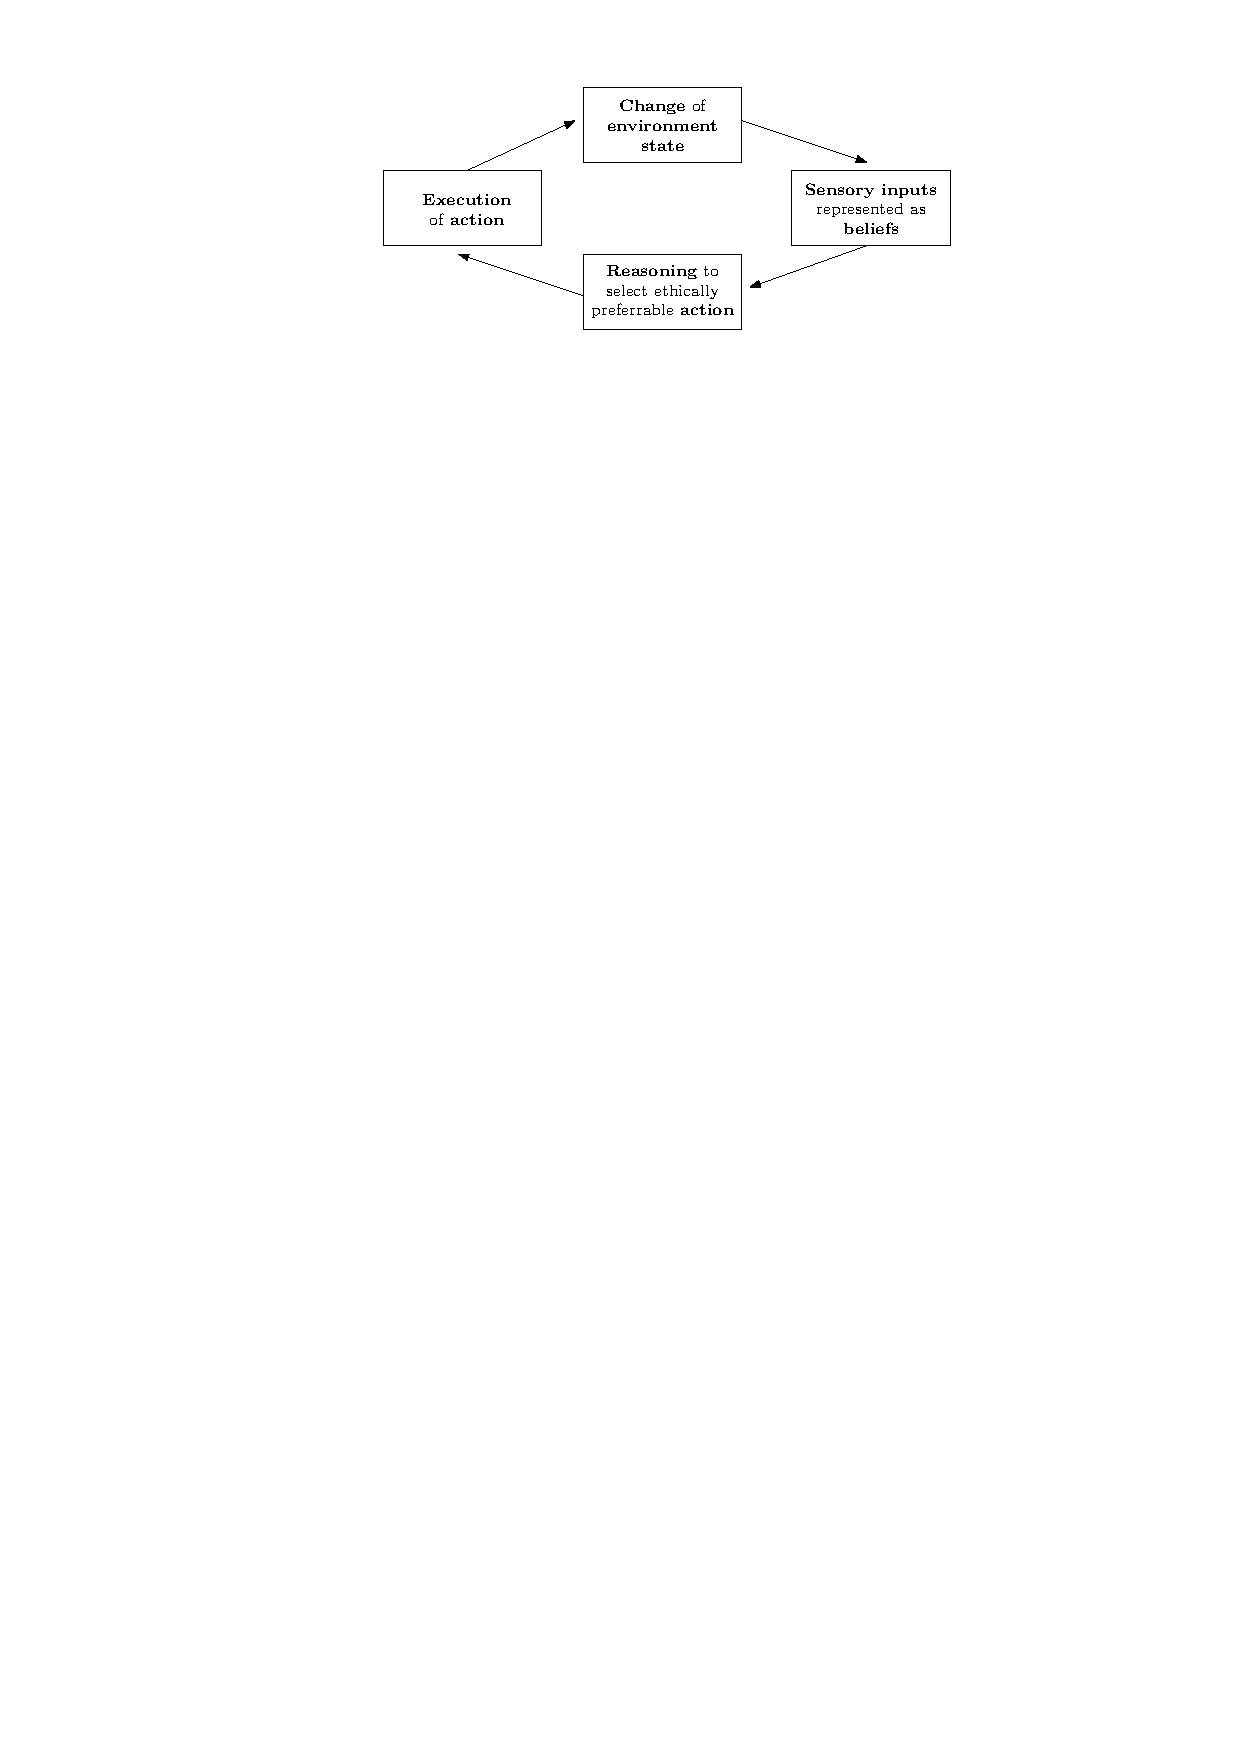
\includegraphics[width=0.8\textwidth]{figures/reason_cycl.pdf}
	\caption{Reasoning cycle of \gls{bdi} agent (adapted from \cite{bremner2019})}
	\label{reasoning}
\end{figure} 


\textbf{Second Example:}
An example of a hybrid architecture can be seen in Figure \ref{hybride_arch}.
\begin{figure}[ht]
	\centering
  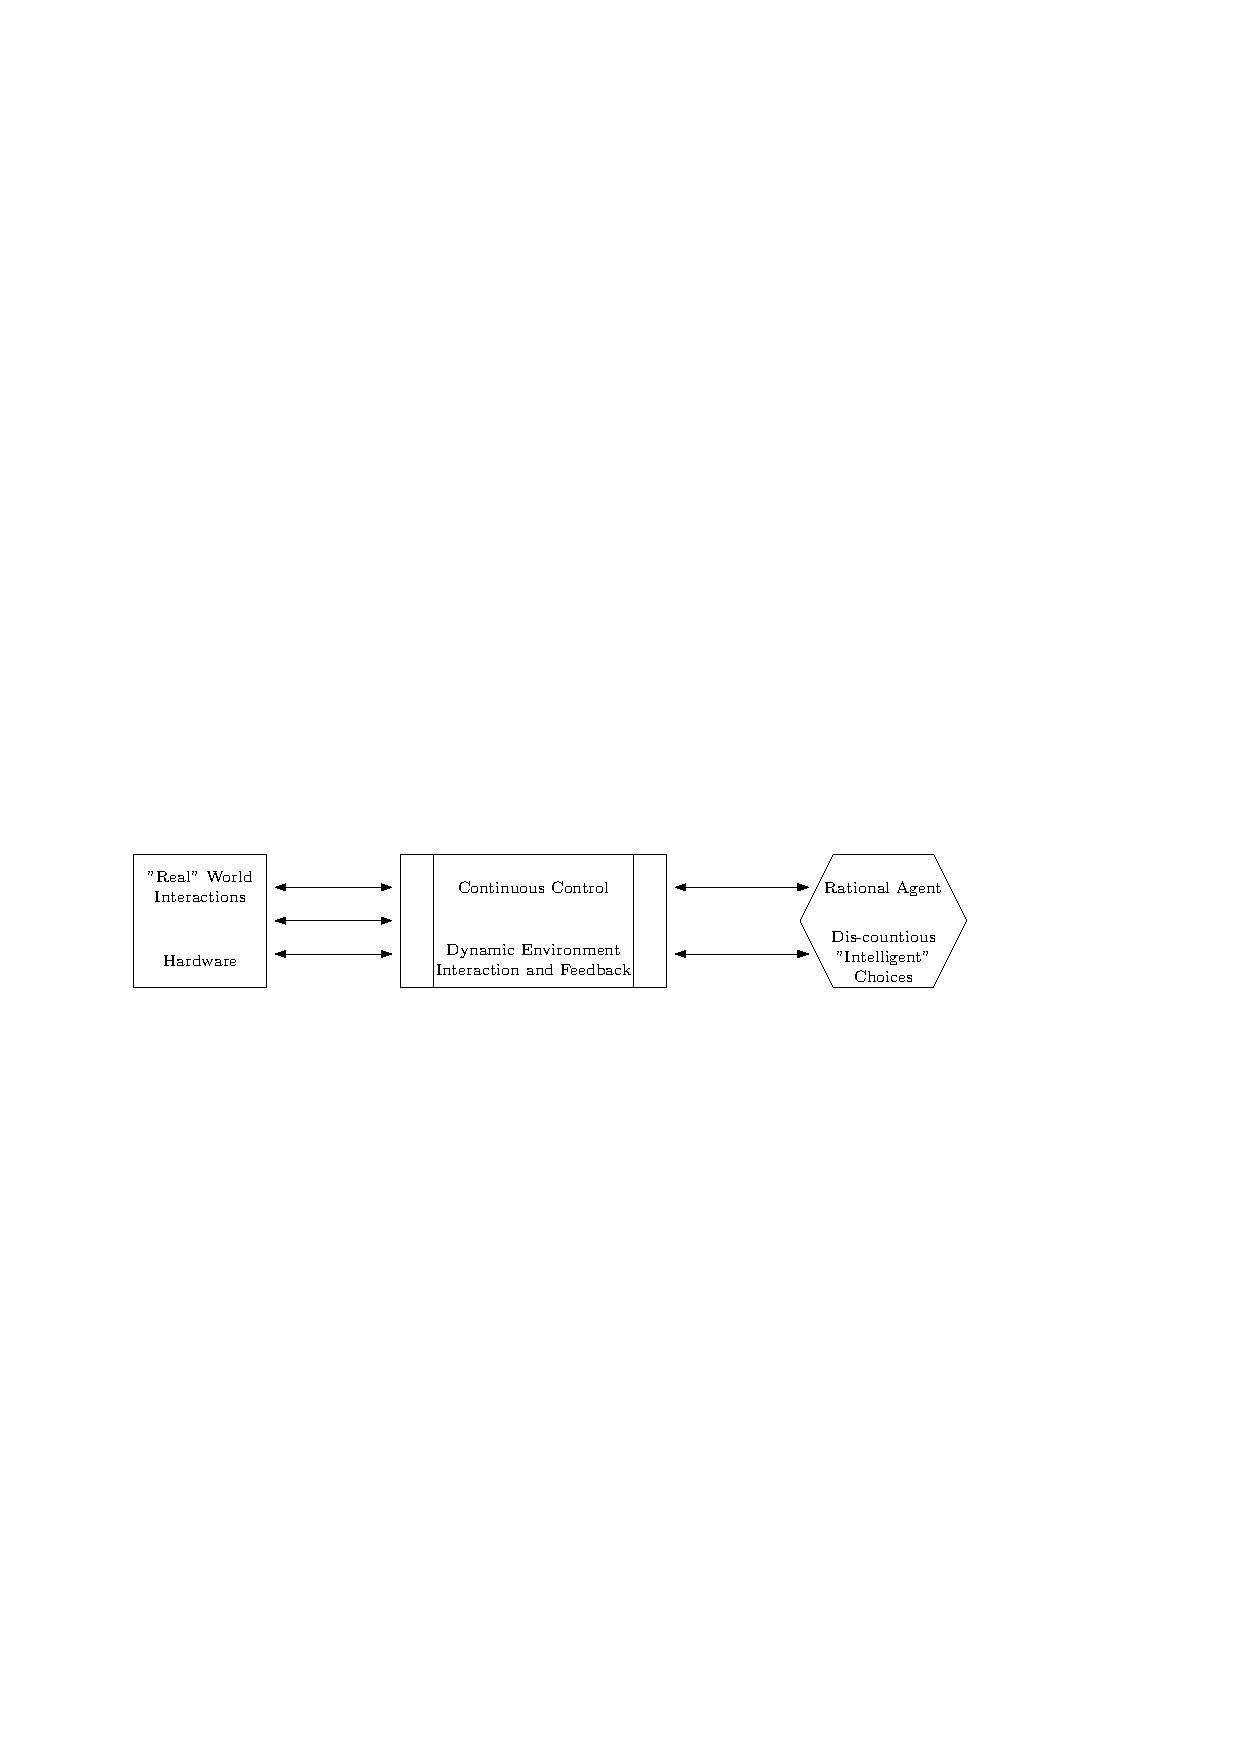
\includegraphics[width=1\textwidth]{figures/hybrid_arch.pdf}
	\caption{Typical hybrid agent architecture \citep{dennis2016}}
	\label{hybride_arch}
\end{figure}



\subsubsection{Examples of tables:}

\textbf{First Example:}
These examples are presented in Table \ref{example_list}. 
%\begin{landscape}
\renewcommand*{\arraystretch}{1.3}
{\footnotesize
\begin{longtable}{ccc}
\caption{List of example beliefs, duties and actions}
			\label{example_list} 
			\cr
			\toprule 
			\centering 
%1. header
{\centering\textbf{Beliefs}} & 
{\centering\textbf{Duties}} & {\centering\textbf{Actions}} \\ \toprule
\endhead
{\parbox{4cm}{low battery}}  & {\parbox{5cm}{maximize honor commitments}}  & {\parbox{5cm}{\emph{charge} robots battery}}  \\  %\specialrule{0.0em}{0.0em}{0.0em}

{\parbox{4cm}{fully charged}}  & {\parbox{5cm}{maximize maintain readiness}}  & {\parbox{5cm}{\emph{remind} patient to take medicine}}  \\  %\specialrule{0.0em}{0.7em}{0.7em}

{\parbox{4cm}{medication reminder time}}  & {\parbox{5cm}{maximize good to patient}}  & {\parbox{5cm}{\emph{engage} with patient}}  \\  %\specialrule{0.0em}{0.7em}{0.7em}

{\parbox{4cm}{reminded}}  & {\parbox{5cm}{maximize respect autonomy}}  & {\parbox{5cm}{\emph{warn} patient }}  \\  %\specialrule{0.0em}{0.7em}{0.7em}

{\parbox{4cm}{refused medication}}  & {\parbox{5cm}{minimize harm to patient}}  & {\parbox{5cm}{\emph{notify} an overseer}}  \\  %\specialrule{0.0em}{0.7em}{0.7em}

{\parbox{4cm}{no interaction}}  & {\parbox{5cm}{minimize non-interaction}}  & {\parbox{5cm}{\emph{return} to seek task position}}  \\  %\specialrule{0.0em}{0.7em}{0.7em}
\bottomrule
\end{longtable}
} 


\textbf{Second Example with colored cells:}
%\begin{landscape}
\renewcommand*{\arraystretch}{1.3}
{\scriptsize
\begin{longtable}{ccccccc}
\caption{Example list of actions and duty satisfaction/violation values}
			\label{action_example} 
			\cr
			\toprule 
			\centering 
%1. header
{\parbox{1cm}{action}} & {\parbox{1.8cm}{Max honor commitments}} & {\parbox{1.8cm}{Max maintain readiness}} & {\parbox{1.4cm}{Min harm to patient}} & {\parbox{1.4cm}{Max good to patient}} & {\parbox{1.5cm}{Min non-interaction}} & {\parbox{1.6cm}{Max respect autonomy}} \\ \toprule
%{\centering\textbf{Beliefs}} & 
%{\centering\textbf{Duties}} & {\centering\textbf{Actions}} \\ \toprule
\endhead
\multicolumn{1}{l}{charge}  & -1  & \cellcolor{SeaGreen} 1 & 0 & -1 & 0 & 0\\ 
\multicolumn{1}{l}{\textbf{remind}} & \cellcolor{SeaGreen} 1 & -1 & 0& -1 & 0 & 0\\
\multicolumn{1}{l}{engage} & -1 & -1 & 0 & -1 & 0 & 0\\
\multicolumn{1}{l}{warn} & -1 & 0 & 0 & -1 & 0 & -1\\
\multicolumn{1}{l}{notify} & -1 & 0 & 0 & -1 & 0 & -2\\
\multicolumn{1}{l}{seek task} & -1 & -1 & 0 & \cellcolor{SeaGreen} 1 & 0 & 0\\

\bottomrule
\end{longtable}
} 
\newpage

\textbf{Third Example with colored cells and explanation of the table:}

%\begin{landscape}
\renewcommand*{\arraystretch}{1.3}
{\scriptsize
\begin{longtable}{ccccccc}
\caption{Comparison of EthIRL and EthLog}
			\label{comparison} 
			\cr
			\toprule 
			\centering 
%1. header
{\parbox{1.5cm}{Approach}} & {\parbox{1.8cm}{Ethical Reasoning}} & {\parbox{1.7cm}{Significant Autonomy}} & {\parbox{1.7cm}{Interactivity}} & {\parbox{1.7cm}{Adaptability}} & {\parbox{1.7cm}{Transparency}} & {\parbox{1.7cm}{Responsibility}}  \\ \toprule
%{\centering\textbf{Beliefs}} & 
%{\centering\textbf{Duties}} & {\centering\textbf{Actions}} \\ \toprule
\endhead
\multicolumn{1}{l}{EthIRL}  & \cellcolor{Orchid!50} O  & \cellcolor{SeaGreen!50} \checkmark & \cellcolor{SeaGreen!50} \checkmark & \cellcolor{SeaGreen!50} \checkmark & \cellcolor{Red!30} X &  \cellcolor{Red!30} X\\ 
\multicolumn{1}{l}{EthLog}  & \cellcolor{SeaGreen!50} \checkmark  &\cellcolor{SeaGreen!50} \checkmark & \cellcolor{SeaGreen!50} \checkmark &\cellcolor{SeaGreen!50} \checkmark & \cellcolor{SeaGreen!50} \checkmark & \cellcolor{Orchid!50} O\\ 
\bottomrule
\multicolumn{6}{l}{\checkmark = Fulfillment, O = Partial Fulfillment, X = Violation} \\
\end{longtable}
}

Table \ref{comparison} summarizes the comparison of EthIRL and EthLog with respect to the different theoretical requirements for explicit ethical agency. Here, it is visible that the EthLog architecture outperforms EthIRL in three requirements: ethical reasoning, transparency and responsibility where EthIRL is not superior to EthLog in any of the other requirements. Therefore, it can be concluded that the EthLog approach is preferable to the EthIRL approach. In this theoretical analysis, the main shortcomings of the EthIRL approach are possible data bias of expert demonstrations, temporal complex norms and lack of transparency making it difficult to apply the concept of shared responsibility. Some extensions can be made to the \gls{dqn} and maximum entropy \gls{irl} approach to ensure a more accurate exploration of the state space $S$. Mechanisms for balancing decision-making with learning about the true underlying values can be fostered by extending the proposed architecture to the case of partially observable MDPs, e.g., by learning belief representations as stated in \cite{gangwani2020learning}. However, the missing concepts of transparency and responsibility are crucial to the evaluation if ethical agency can be ascribed to the EthIRL agent. This problem stays unresolved because no satisfying answer can be found that can be incorporated into the architecture. Even though the EthIRL agent competes well in some of the more technical categories, it has too many shortcomings and, thus, cannot be categorized as ethical agent. The main drawbacks of the EthLog approach are the hand-designed training data which are prone to bias and errors. This makes a full application of the concept of shared responsibility difficult. Another issue may occur when the cases taken for the training of the ethical reasoning module are fuzzy or noisy. This can be solved by combining \gls{ilp} with function approximation techniques like NNs, as proposed in \cite{evans2018learning, payani2019inductive}. The issue of biased data is a general challenge in the machine learning domain and some techniques have been proposed to tackle this problem. This includes bias detection by determining the relative feature importance proposed by \cite{pascanu2017}. However, a detailed description of such solutions is out of the scope of this thesis. \\


\subsubsection{Examples of math equations:}

\textbf{First Example:}

\begin{equation}
   IG(D,a) = H(D) - \sum_v \frac{|D_v|}{|D|}H(D_v)
\end{equation}{}

where the information gain $IG(D,a)$ from splitting the data set $D$ using the feature $a$ is defined as entropy $H(D)$ of the training examples minus the expected average entropy over each set of attributes with a particular value $v$ in a feature. This is then multiplied with the entropy of a particular data set containing the value $D_v$. The information gain is calculated for each remaining feature where the feature with the largest information gain is used to split the set $D$ in the current iteration \citep{wang2017improvement}.

\subsubsection{Example of how pseudocode should look like in a thesis:}
\begin{algorithm}[H]
\caption{ID3 Algorithm}\label{alg_id3}
\begin{algorithmic}[1]
\Input set of features $A$, set of training instances $D$
\Output decision-tree 
\If{all instances in $D$ have same class $C$} \\
\hspace{0.5cm} \Return{a decision-tree consisting of a leaf node with label $C$}
\ElsIf{$A$ is empty}\\
\hspace{0.5cm} \Return{a decision-tree with leaf node and label of the target level in $D$} 
\ElsIf{$D$ is empty}\\
\hspace{0.5cm} \Return{decision-tree with label of majority target level of parent node} 
%a decision tree comprising of a leaf node with the label the majority target level of the data set of the immediate parent node
\Else
\State $a[best] \leftarrow \underset{a \in A}{\arg\max} IG(D,a)$
\State make new node $Node_{a[best]}$ and label it with $a[best]$
\State partition $D$ using $a[best]$ from $A$
\State remove $a[best]$ from $A$
\EndIf 
\For{each partition $D_v$ of $D$}
\State grow branch from $Node_{a[best]}$ to the decision-tree created by re-running ID3 with $D = D_v$
\EndFor
\end{algorithmic}
\end{algorithm}

Algorithm \ref{alg_id3} shows the pseudocode description from the ID3 algorithm adapted from \cite{kelleher2015fundamentals} and consists of two parts: in the first part (lines 1-6), the algorithm terminates the current path in the tree by adding a new node. Alternatively, in the second part (line 7-13), a node is initialized where the algorithm extends the current path by adding an interior node to the tree by growing the branches of this node as a result of repeatedly re-running the algorithm....






% Bibliography
\newpage
\addcontentsline{toc}{section}{References}
\bibliographystyle{references/kbib}
\bibliography{references/ref}

% Declaration of Originality
\newpage
\thispagestyle{empty}
\section*{Declaration of Originality:}
%\section{Erklärung zur eigenständigen Arbeit }
%I declare that I wrote my thesis by myself and that I did not use other references or auxiliary aids which I did not quote. Every passage, which I took word by word or analogous out of other sources, has been marked properly. The work or a similar work was not submitted before to another examination office.

I promise, that I wrote my thesis by myself and that I did not use other references or auxiliary aids, which I did not quote. Every passage, which I took word by word or analogous out of other sources, have been marked properly. The work or an similar work was not handed before at another examination office.

~~~\\

\vspace{5cm}

$\overline{~~~~~~~~~\mbox{Your location, add date of submission, add your name (Matrnr: )}~~~~~~~~~}$




\end{spacing}
\end{document}